\documentclass{beamer}
%
% Choose how your presentation looks.
%
% For more themes, color themes and font themes, see:
% http://deic.uab.es/~iblanes/beamer_gallery/index_by_theme.html
%
\mode<presentation>
{
  \usetheme{default}      % or try Darmstadt, Madrid, Warsaw, ...
  \usecolortheme{default} % or try albatross, beaver, crane, ...
  \usefonttheme{default}  % or try serif, structurebold, ...
  \setbeamertemplate{navigation symbols}{}
  \setbeamertemplate{caption}[numbered]
} 

\usepackage[english]{babel}
\usepackage[utf8]{inputenc}
\usepackage[T1]{fontenc}

\title[Escalonamento]{Escalonamento e existência de soluções}
\author{MAP 2110 - Diurno}
\institute{IME USP}
\date{28 de abril}

\begin{document}

\begin{frame}
  \titlepage
\end{frame}

% Uncomment these lines for an automatically generated outline.
%\begin{frame}{Outline}
%  \tableofcontents
%\end{frame}


\section{Sistemas Lineares}

\begin{frame}{Matriz na forma escalonada}

 Vamos estudar o que acontece quando aplicamos o algoritmo da Eliminação de Gauss em sistemas
 lineares de qualquer dimensão, isto é, com $n$ incógnitas e $m$ equações.
   \begin{block}{Sistema Linear}
     \begin{gather*}
      a_{11}x_1 + a_{12}x_2 + \cdots + a_{1n}x_n = b_1 \\
      a_{21}x_1 + a_{22}x_2 + \cdots + a_{2n}x_n = b_2 \\
      \vdots \\
      a_{m1}x_1 + a_{m2}x_2 + \cdots + a_{mn}x_n = b_m \\
    \end{gather*}
  \end{block}
\end{frame}

\begin{frame}{Exemplo}
  Vamos ver o seguinte exemplo com $4$ equações e $5$ incógnitas.

  \begin{align*}
    x_1 + x_2 - x_3 + 2x_4 +x_5 &= a \\
    2x_1 +  x_3 + x_4 +3x_5 &= b \\
    3x_1 + x_2  + 3x_4 +4x_5 &= c \\
    x_1 -x_2 + x_4  &= d\\
  \end{align*}
  
\end{frame}

\begin{frame}{Matriz aumentada do sistema}
  Matriz aumentada = matriz dos coeficientes junto com os elemntos do lado direito da equação
$$
 \left[ \begin{array}{ccccc|c}
    x_1 & x_2 & x_3 & x_4 & x_5 & \\ \hline
    1 & 1 & -1 & 2 & 1 & a \\ 
    2 & 0 & 1 &1 & 3 & b \\
    3 & 1 & 0 & 3 & 4 & c \\
    1 & -1 & 0 & 1 & 0 & d
    \end{array}\right]
$$
  

\end{frame}
\begin{frame}
  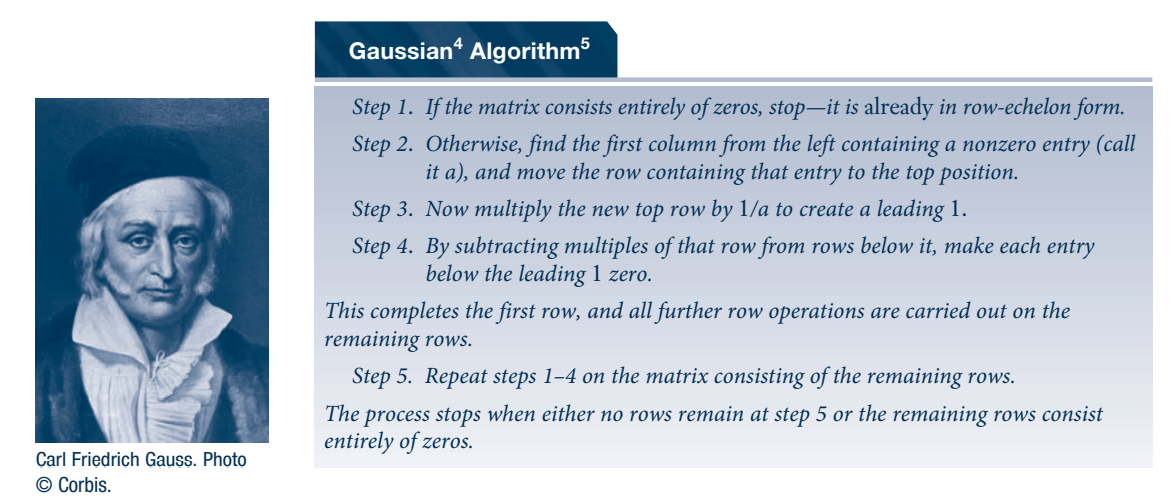
\includegraphics[scale=0.4]{gausselim.png}
\end{frame}

\begin{frame}{Aplicando o método de Eliminação}

  $$
  \left[ \begin{array}{ccccc|c}
     \textcolor{red}{1} & 1 & -1 & 2 & 1 & a \\ 
     2 & 0 & 1 &1 & 3 & b \\
     3 & 1 & 0 & 3 & 4 & c \\
     1 & -1 & 0 & 1 & 0 & d
     \end{array}\right]
 $$
Faremos as operações elementares:
\begin{gather*}  
  L_2 = L_2-2L_1 \\
  L_3 = L_3 -3L_1 \\
  L_4 = L_4 - L_1
\end{gather*}
\end{frame}


\begin{frame}{Aplicando o método de Eliminação- 2 }
  $$
  \left[ \begin{array}{ccccc|c}
     1 & 1 & -1 & 2 & 1 & a \\ 
      0 & \textcolor{red}{-2} & 3 &-3 & 1 & b-2a \\
     0 & -2 & 3 & -3 & 1 & c-3a \\
     0 & -2 & 1 & -1 & -1 & d -a
     \end{array}\right]
 $$
 \begin{gather*}  
  L_3 = L_3- L_2 \\
  L_4 = L_4 - L_2
\end{gather*}
\end{frame}

\begin{frame}{Aplicando o método de Eliminação- 3 }
  $$
  \left[ \begin{array}{ccccc|c}
     1 & 1 & -1 & 2 & 1 & a \\ 
      0 & -2 & 3 &-3 & 1 & b-2a \\
     0 & 0 & 0 & 0 & 0 & c-b-a \\
     0 & 0 & -2 & 2 & -2 & d -b + a
     \end{array}\right]
 $$
 \begin{gather*}  
  L_3 = L_4 \\
  L_4 =L_3
\end{gather*}
\end{frame}

\begin{frame}

  $$
  \left[ \begin{array}{ccccc|c}
     \textcolor{red}{1} & 1 & -1 & 2 & 1 & a \\ 
      0 & \textcolor{red}{-2} & 3 &-3 & 1 & b-2a \\
      0 & 0 & \textcolor{red}{-2} & 2 & -2 & d -b + a \\
      0 & 0 & 0 & 0 & 0 & c-b-a \\
     \end{array}\right]
 $$
Na forma escalonada teríamos
\end{frame}

\begin{frame}{Forma escalonada}

 $$
  \left[ \begin{array}{ccccc|c}
     \textcolor{red}{1} & 1 & -1 & 2 & 1 & a \\ 
      0 & \textcolor{red}{1} & -3/2 &3/2 & -1/2 & (2a-b)/2 \\
      0 & 0 & \textcolor{red}{1} & -1 & 1 & (b - a -d)/2 \\
      0 & 0 & 0 & 0 & 0 & c-b-a \\
     \end{array}\right]
 $$

\end{frame}



\begin{frame}{podemos fazer o escalonamento usando operações elementares diferentes}
  Vamos partir do segundo passo do escalonamento acima:

  $$
  \left[ \begin{array}{ccccc|c}
     1 & 1 & -1 & 2 & 1 & a \\ 
      0 & -2 & 3 &-3 & 1 & b-2a \\
     0 & -2 & 3 & -3 & 1 & c-3a \\
     0 & -2 & 1 & -1 & -1 & d -a
     \end{array}\right]
 $$
 E fazer agora primeiro a troca da linha 4 e 2 
 \begin{gather*}  
  L_2 = L_4 \\
  L_4 = L_2
\end{gather*}

\end{frame}
$$
\left[ \begin{array}{ccccc|c}
   1 & 1 & -1 & 2 & 1 & a \\ 
   0 & \textcolor{red}{-2} & 1 & -1 & -1 & d -a\\
  0 & -2 & 3 & -3 & 1 & c-3a \\
   0 & -2 & 3 &-3 & 1 & b-2a 
\end{array}\right]
$$
\begin{gather*}
  L_3 = L_3 - L_2 \\
  L_4 = L_4 -L_2
\end{gather*}

\begin{frame}
   
  $$
  \left[ \begin{array}{ccccc|c}
     1 & 1 & -1 & 2 & 1 & a \\ 
     0 & -2 & 1 & -1 & -1 & d -a\\
    0 & 0 & 2 & -2 & 2 & c -d-2a \\
     0 & 0 & 2 &-2 & 2 & b-d -a 
  \end{array}\right]
  $$
  \begin{gather*}
    L_4=L4-L_3
  \end{gather*}


\end{frame}



\begin{frame}{ }
  $$
  \left[ \begin{array}{ccccc|c}
     1 & 1 & -1 & 2 & 1 & a \\ 
     0 & -2 & 1 & -1 & -1 & d -a\\
    0 & 0 & 2 & -2 & 2 & c -d-2a \\
     0 & 0 & 0 &0 & 0 & b +a -c 
  \end{array}\right]
  $$
\end{frame}



\begin{frame}{ }
  $$
  \left[ \begin{array}{ccccc|c}
     1 & 1 & -1 & 2 & 1 & a \\ 
     0 & 1 & -1/2 & 1/2 & 1/2 & (a-d)/2\\
    0 & 0 & 1 & -1 & 1 & (c -d-2a)/2 \\
     0 & 0 & 0 &0 & 0 & b +a -c 
  \end{array}\right]$$
  \pause 
  $$\neq 
  \textcolor{green}{\left[ \begin{array}{ccccc|c}
    {1} & 1 & -1 & 2 & 1 & a \\ 
     0 & {1} & -3/2 &3/2 & -1/2 & (2a-b)/2 \\
     0 & 0 & {1} & -1 & 1 & (b - a -d)/2 \\
     0 & 0 & 0 & 0 & 0 & c-b-a \\
    \end{array}\right]}
  $$
\end{frame}

\begin{frame}{Forma escalonada reduzida}
  Este método também é conhecido como algoritmo de Gauss Jordan.
  Vamos começar com a segunda versão do processo de escalonamento:
  $$
  \left[ \begin{array}{ccccc|c}
     1 & 1 & -1 & 2 & 1 & a \\ 
     0 & 1 & -1/2 & 1/2 & 1/2 & (a-d)/2\\
    0 & 0 & 1 & -1 & 1 & (c -d-2a)/2 \\
     0 & 0 & 0 &0 & 0 & b +a -c 
  \end{array}\right]$$
  Continuando com as operações elementares
  \begin{gather*}
    L_2 = L_2 + 1/2*L_3 \\
    L_1 = L_1 + L_3
  \end{gather*}

\end{frame}

\begin{frame}{}
  $$
  \left[ \begin{array}{ccccc|c}
     1 & 1 & 0 & 1 & 2 & (c-d)/2 \\ 
     0 & 1 & 0 & 0 & 1 & (c-3d)/4\\
    0 & 0 & 1 & -1 & 1 & (c -d-2a)/2 \\
     0 & 0 & 0 &0 & 0 & b +a -c 
  \end{array}\right]$$
  \begin{gather*}
    L_1 = L_1 - L_2
  \end{gather*}
\end{frame}

\begin{frame}{}
  $$
  \left[ \begin{array}{ccccc|c}
     1 & 0 & 0 & 1 & 1 & (d+c)/4 \\ 
     0 & 1 & 0 & 0 & 1 & (c-3d)/4\\
    0 & 0 & 1 & -1 & 1 & (c -d-2a)/2 \\
     0 & 0 & 0 &0 & 0 & b +a -c 
  \end{array}\right]$$
  Esta é a forma escalonada reduzida da matriz
\end{frame}

\begin{frame}{O processo de Jordan com a segunda Matriz escalonada}
  $$
  \left[ \begin{array}{ccccc|c}
    {1} & 1 & -1 & 2 & 1 & a \\ 
     0 & {1} & -3/2 &3/2 & -1/2 & (2a-b)/2 \\
     0 & 0 & {1} & -1 & 1 & (b - a -d)/2 \\
     0 & 0 & 0 & 0 & 0 & c-b-a \\
    \end{array}\right]
  $$
\begin{gather*}
  L_2 =L_2 + 3/2*L_3 \\
  L_1 =L_1 + L_3
\end{gather*}

\end{frame}


\begin{frame}
  $$
  \left[ \begin{array}{ccccc|c}
    {1} & 1 & 0 & 1 & 2 & (b+a-d)/2 \\ 
     0 & {1} & 0 &0 & 1 & (a+b-3d)/4 \\
     0 & 0 & {1} & -1 & 1 & (b - a -d)/2 \\
     0 & 0 & 0 & 0 & 0 & c-b-a \\
    \end{array}\right]
  $$
\begin{gather*}
  L_1 =L_1 - L_2
\end{gather*}

\end{frame}


\begin{frame}
  $$
  \left[ \begin{array}{ccccc|c}
     1 & 0 & 0 & 1 & 1 & (b+a +d)/4 \\ 
     0 & 1 & 0 &0 & 1 & (a+b-3d)/4 \\
     0 & 0 & 1 & -1 & 1 & (b - a -d)/2 \\
     0 & 0 & 0 & 0 & 0 & c-b-a \\
    \end{array}\right]
  $$

\end{frame}

\begin{frame}{Comparando as formas reduzidas}
  Obtidas com diferentes operações elementares.
  $$
  \left[ \begin{array}{ccccc|c}
     1 & 0 & 0 & 1 & 1 & (b+a+d)/4 \\ 
     0 & 1 & 0 &0 & 1 & (a+b-3d)/4 \\
     0 & 0 & 1 & -1 & 1 & (b - a -d)/2 \\
     0 & 0 & 0 & 0 & 0 & c-b-a \\
    \end{array}\right]
  $$ 

 $$
  \left[ \begin{array}{ccccc|c}
     1 & 0 & 0 & 1 & 1 & (d+c)/4 \\ 
     0 & 1 & 0 & 0 & 1 & (c-3d)/4\\
    0 & 0 & 1 & -1 & 1 & (c -d-2a)/2 \\
     0 & 0 & 0 &0 & 0 & b +a -c 
  \end{array}\right]$$
\end{frame}
   
\end{document}
